\documentclass[a4paper, 12pt]{article}
\usepackage{pgfplots}
\usepackage{mathtools}

%% Listings With Code-Styling and Grey Background
\usepackage{float}
\usepackage{listings} 
\usepackage{xcolor}
\usepackage{mdframed}
\usepackage{graphicx}
\definecolor{code-gray}{gray}{0.93}

%% Custom FSM's
\usepackage{tikz}
\usetikzlibrary{automata, positioning, arrows, backgrounds}
\tikzset{very thick, ->, >=stealth', node distance=6cm, every state/.style={thick, fill=gray!10}, initial text=$ $}

%% Automatic Word Formatting
\usepackage{xspace}
\newcommand*{\Vivado}{\textit{Vivado}\xspace} % Italicize Vivado
\newcommand*{\SV}{\textbf{SystemVerilog}\xspace} % Bold SystemVerilog

%% Clickable links in the output PDF
\usepackage{hyperref}
\hypersetup{colorlinks=true, linktoc=all, linkcolor=black}

%% Figure Numbering Within Sections
\let\counterwithout\relax
\let\counterwithin\relax
\usepackage{chngcntr}
\counterwithin{figure}{section}

%% Macros for logic timing diagrams
\newcounter{wavenum}
\setlength{\unitlength}{1cm}
% advance clock one cycle, not to be called directly
\newcommand*{\clki}{
  \draw (t_cur) -- ++(0,.3) -- ++(.5,0) -- ++(0,-.6) -- ++(.5,0) -- ++(0,.3)
    node[time] (t_cur) {};
}
\newcommand*{\bitvector}[3]{
  \draw[fill=#3] (t_cur) -- ++( .1, .3) -- ++(#2-.2,0) -- ++(.1, -.3)
                         -- ++(-.1,-.3) -- ++(.2-#2,0) -- cycle;
  \path (t_cur) -- node[anchor=mid] {#1} ++(#2,0) node[time] (t_cur) {};
}
% \known{val}{length}
\newcommand*{\known}[2]{
    \bitvector{#1}{#2}{white}
}
% \unknown{length}
\newcommand*{\unknown}[2][XXX]{
    \bitvector{#1}{#2}{black!20}
}
% \bit{1 or 0}{length}
\newcommand*{\bit}[2]{
  \draw (t_cur) -- ++(0,.6*#1-.3) -- ++(#2,0) -- ++(0,.3-.6*#1)
    node[time] (t_cur) {};
}
% \unknownbit{length}
\newcommand*{\unknownbit}[1]{
  \draw[ultra thick,black!50] (t_cur) -- ++(#1,0) node[time] (t_cur) {};
}
% \nextwave{name}
\newcommand{\nextwave}[1]{
  \path (0,\value{wavenum}) node[left] {#1} node[time] (t_cur) {};
  \addtocounter{wavenum}{-1}
}
% \clk{name}{period}
\newcommand{\clk}[2]{
    \nextwave{#1}
    \FPeval{\res}{(\wavewidth+1)/#2}
    \FPeval{\reshalf}{#2/2}
    \foreach \t in {1,2,...,\res}{
        \bit{\reshalf}{1}
        \bit{\reshalf}{0}
    }
}

% \begin{wave}[clkname]{num_waves}{clock_cycles}
\newenvironment{wave}[3][clk]{
  \begin{tikzpicture}[draw=black, yscale=.7,xscale=1]
    \tikzstyle{time}=[coordinate]
    \setlength{\unitlength}{1cm}
    \def\wavewidth{#3}
    \setcounter{wavenum}{0}
    \nextwave{#1}
    \foreach \t in {0,1,...,\wavewidth}{
      \draw[dotted] (t_cur) +(0,.5) node[above] {t=\t} -- ++(0,.4-#2);
      \clki
    }
}{\end{tikzpicture}}

%$ Specific Line Breaks
% See https://tex.stackexchange.com/questions/26174/ for details
\usepackage[british]{babel} 

%% Page Margins
\usepackage[margin=1.00in]{geometry}

%% Beginning of Document
\begin{document}
\counterwithin{lstlisting}{section} % Listings are numbered within sections
% Title
\title{ECE 440 - Homework \#4}
\author{Collin Heist}
\date{\today}
\maketitle

% Table of Content and Listings
\pagenumbering{arabic}

% Beginning of Report
\section{Wrapper Module Block Diagram}
\begin{figure}[h]
\hspace*{-0.75cm}
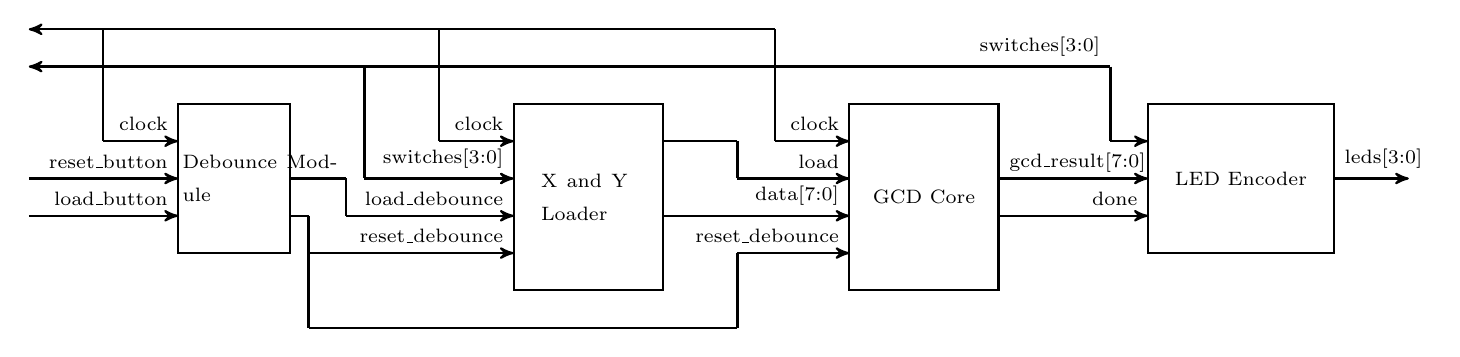
\begin{tikzpicture}[thick, node distance=0.5cm]
\def \scale {18/38}

\draw[<-] (0, -0) -- (20*\scale, -0);
\draw[<-] (0, -1*\scale) -- (29*\scale, -1*\scale) node[above left]{\scriptsize{switches[3:0]}};
\draw[-] (2*\scale, -0) -- (2*\scale, -3*\scale);
\draw[->] (2*\scale, -3*\scale) -- (4*\scale, -3*\scale) node[above left]{\scriptsize{clock}};
\draw[->] (0, -4*\scale) -- (4*\scale, -4*\scale) node[above left]{\scriptsize{reset\_button}};
\draw[->] (0, -5*\scale) -- (4*\scale, -5*\scale) node[above left]{\scriptsize{load\_button}};
\draw (4*\scale, -2*\scale) rectangle (7*\scale, -6*\scale) node[midway, text width=2cm, xshift=0.35cm]{\scriptsize{Debounce Module}};
\draw[-] (11*\scale, 0*\scale) -- (11*\scale, -3*\scale);
\draw[->] (11*\scale, -3*\scale) -- (13*\scale, -3*\scale) node[above left]{\scriptsize{clock}};
\draw[-] (9*\scale, -1*\scale) -- (9*\scale, -4*\scale);
\draw[->] (9*\scale, -4*\scale) -- (13*\scale, -4*\scale) node[above left]{\scriptsize{switches[3:0]}};
\draw[-] (7*\scale, -4*\scale) -- (8.5*\scale, -4*\scale);
\draw[-] (8.5*\scale, -4*\scale) -- (8.5*\scale, -5*\scale);
\draw[->] (8.5*\scale, -5*\scale) -- (13*\scale, -5*\scale) node[above left]{\scriptsize{load\_debounce}};
\draw[-] (7*\scale, -5*\scale) -- (7.5*\scale, -5*\scale);
\draw[-] (7.5*\scale, -5*\scale) -- (7.5*\scale, -8*\scale);
\draw[-] (7.5*\scale, -8*\scale) -- (19*\scale, -8*\scale);
\draw[->] (7.5*\scale, -6*\scale) -- (13*\scale, -6*\scale) node[above left]{\scriptsize{reset\_debounce}};
\draw (13*\scale, -2*\scale) rectangle (17*\scale, -7*\scale) node[midway, text width=2cm, xshift=0.4cm]{\scriptsize{X and Y Loader}};
\draw[-] (20*\scale, 0) -- (20*\scale, -3*\scale);
\draw[->] (20*\scale, -3*\scale) -- (22*\scale, -3*\scale) node[above left]{\scriptsize{clock}};
\draw[-] (17*\scale, -3*\scale) -- (19*\scale, -3*\scale);
\draw[-] (19*\scale, -3*\scale) -- (19*\scale, -4*\scale);
\draw[->] (19*\scale, -4*\scale) -- (22*\scale, -4*\scale) node[above left]{\scriptsize{load}};
\draw[->] (17*\scale, -5*\scale) -- (22*\scale, -5*\scale) node[above left]{\scriptsize{data[7:0]}};
\draw[-] (19*\scale, -8*\scale) -- (19*\scale, -6*\scale);
\draw[->] (19*\scale, -6*\scale) -- (22*\scale, -6*\scale) node[above left]{\scriptsize{reset\_debounce}};
\draw (22*\scale, -2*\scale) rectangle (26*\scale, -7*\scale) node[midway]{\scriptsize{GCD Core}};
\draw[-] (29*\scale, -1*\scale) -- (29*\scale, -3*\scale);
\draw[->] (29*\scale, -3*\scale) -- (30*\scale, -3*\scale);
\draw[->] (26*\scale, -4*\scale) -- (30*\scale, -4*\scale) node[above left, xshift=3, yshift=-1.5]{\scriptsize{gcd\_result[7:0]}};
\draw[->] (26*\scale, -5*\scale) -- (30*\scale, -5*\scale) node[above left]{\scriptsize{done}};
\draw (30*\scale, -2*\scale) rectangle (35*\scale, -6*\scale) node[midway]{\scriptsize{LED Encoder}};
\draw[->] (35*\scale, -4*\scale) node[above right]{\scriptsize{leds[3:0]}} -- (37*\scale, -4*\scale) ;
\end{tikzpicture}
\end{figure}

In this diagram, the debounce module is a \textbf{SystemVeriog} module provided to us. The X and Y loader component is a synchronous block of logic that allows the user to piece-wise input X and Y, and then sends those values (along with the Load signal) to the GCD core. The done signal is then used, along with the results and the switches in the final LED Encoder block. This block is purely combinational. 

\end{document}